\section{System Model}
\label{sec:model}

\begin{figure}[htp!]
    \centering
    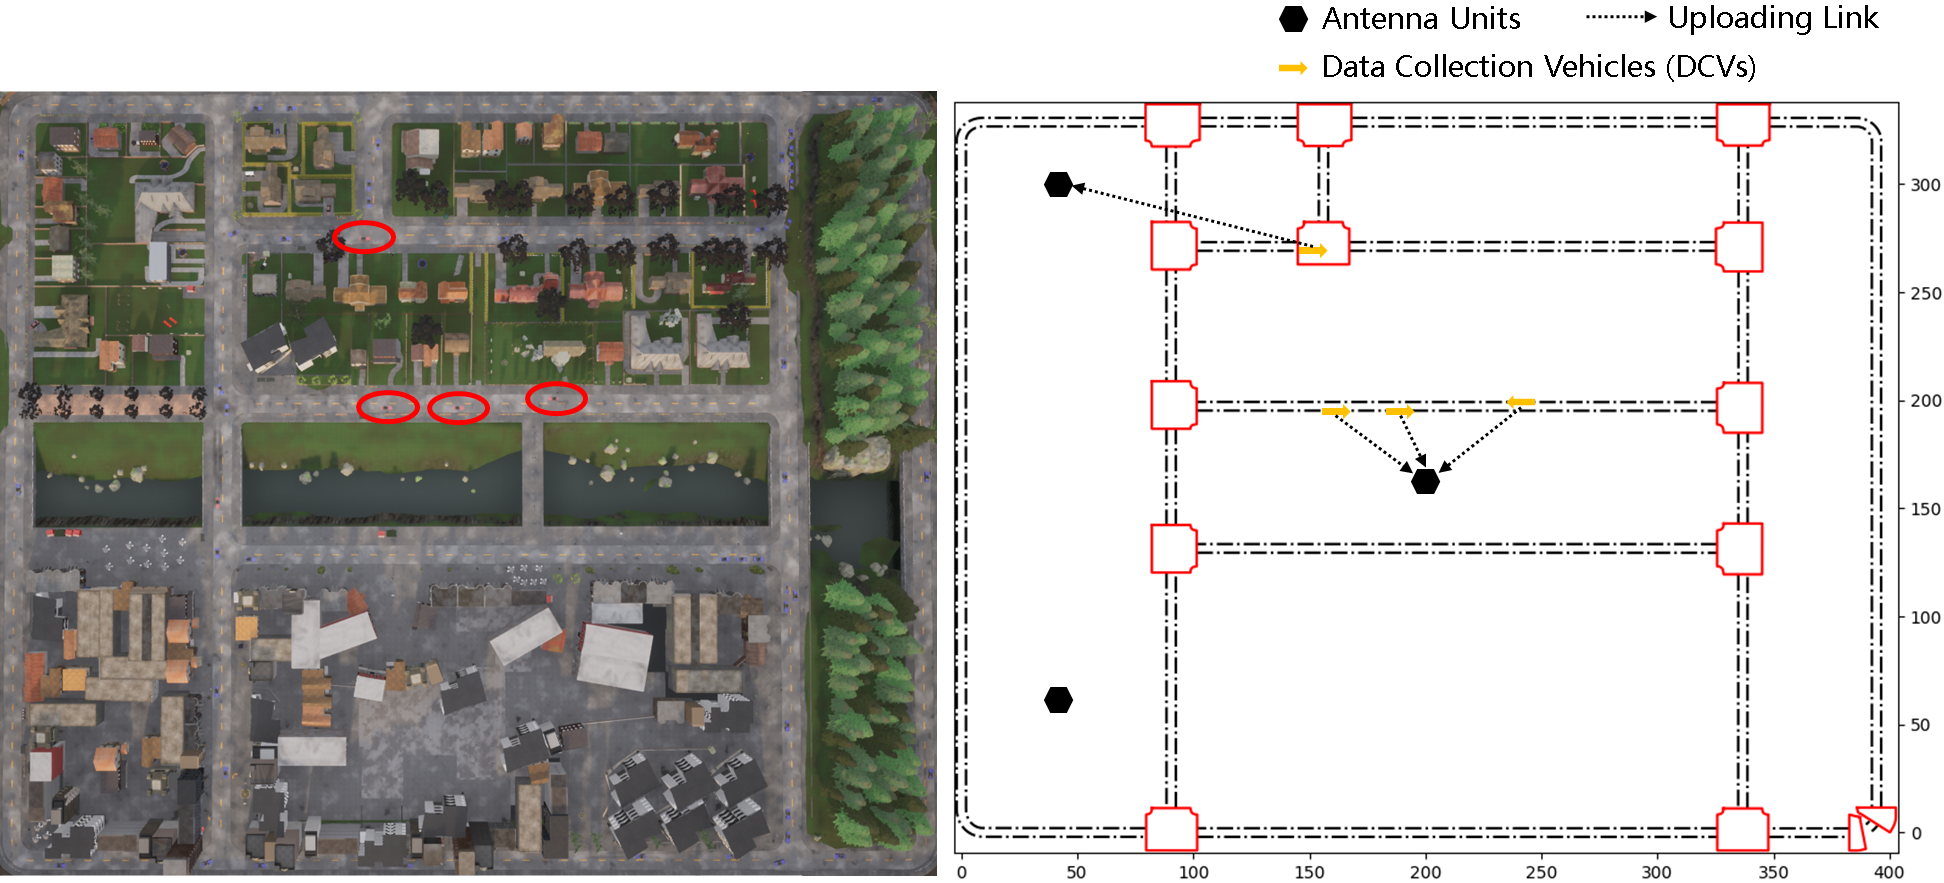
\includegraphics[width=0.45\textwidth]{fig-traffic-demo.png}
    \caption{Illustration of a road map example generated by CARLA.}
    \label{fig:town_map}
\end{figure}

In this paper, the scheduling of model uploading in a vehicular federated learning system is considered, which consists of $M$ {\IAVs} deployed with multi-modal sensors.
Denote the set of {\IAVs} as $\carSet = \set{1, \dots, M}$.
Each {\IAV} collects the sensing data for the cooperative training of a deep neural network, e.g., SECOND \cite{SECOND}, in a federated learning manner \cite{FedAvg}.
This is one of the typical machine learning scenario in the application of autonomous driving as elaborated in \cite{icra21-invs}.
In each training iteration, all the {\IAVs} first train their local models and then upload the trained models to an edge server for model aggregation via cellular uplink.
The aggregated model is then broadcast to the {\IAVs} for local training of next iteration until the convergence.
We particularly consider the uplink transmission scheduling in one iteration, where the {\IAVs}' mobility is exploited to save the transmission energy and suppress the model uploading time.

As an example illustrated in Fig.\ref{fig:town_map}, $M$ {\IAVs} are distributed at different positions of a road network.
They are moving along predetermined routes respectively, but their velocities are time-varying and random.
The route of the $m$-th {\IAV} ($\forall m\in\carSet$) is quantized into a sequence of waypoints denoted as
\begin{align*}
    \tjSet_{m} \define \Paren{ \vec{w}_{m,1}, \dots, \vec{w}_{m,|\tjSet_{m}|} },
\end{align*}
where $\vec{w}_{m,i} \in \domR^2$ denotes the coordinates of the $i$-th waypoint,
$|\tjSet_m|$ denotes the cardinality of $\tjSet_m$.

The system time is organized by time slots, each with a duration of $T_s$ seconds.
In the $t$-th time slot, the location of the $m$-th {\IAV} is denoted as $\vec{d}_{m,t} \in \tjSet_{m}$, and the trajectory of the $m$-th {\IAV} is represented by its locations in all the time slots, denoted by the stochastic process
\begin{align*}
    \vec{L}_{m} \define \Paren{ \vec{d}_{m,1}, \vec{d}_{m,2}, \dots }.
\end{align*}

In this paper, we approximate the trajectories of all {\IAVs} $\set{ \vec{L}_{m} | \forall m\in\carSet }$ as time-invariant Markov chains with the transition matrices
$\set{ \TransD_{m} \in \domR^{|\tjSet_{m}| \times |\tjSet_{m}|} | \forall m\in\carSet }$, where $\vec{D}_{m}$ represents the transition matrix of the $m$-th {\IAV}.
The entries of the transition matrix $\TransD_{m}$ are defined as follows:
\footnote{
    A sufficient number of waypoints is selected for each route, such that the last waypoint is never reached at the end of the model uploading.
    For example, the uploading of the $m$-th {\IAV} always completes before arriving at the waypoint $\vec{w}_{m,|\tjSet_m|}$.
}
\begin{align}
     \Paren{\TransD_{m}}_{i,j} \define \Pr\Bracket{ \vec{w}_{m,j} | \vec{w}_{m,i} }, \forall i,j.
    \label{eqn:trans_mat}
\end{align}

Without loss of generality, the local model training and uploading of the considered iteration starts from the $1$-st time slot.
Due to the heterogeneous computation capabilities of the {\IAVs}, the local training time of the {\IAVs} may be different.
It is assumed that the local training time of the $m$-th {\IAV} is $T_{\text{comp},m}$, and the model consists of $U$ information bits.
Hence, an uplink queue with $U$ information bits is established at the $m$-th {\IAV} since the $(T_{\text{comp},m}+1)$-th time slot.
The period from the $1$-st time slot to the time slot that all the {\IAVs} complete their model uploading is referred to as the \emph{scheduling period} in the remaining of this paper.
Therefore, the length of the actual scheduling period depends on the uplink transmission scheduling policy.

All the {\IAVs} are served via a BS with $Y$ distributed antenna units,
and the locations of the antenna units are denoted as $\vec{b}_1, \dots, \vec{b}_Y$, respectively.
Each {\IAV} delivers its local model to the closest antenna unit, such that the transmission energy can be saved.
The distance between the $m$-th {\IAV} and the receive antenna unit in the $t$-th time slot is denoted as
\begin{align*}
    l_{m,t} = \min_{i=1,2,\dots,Y} \|\vec{d}_{m,t} - \vec{b}_i\|_2.
\end{align*}
In order to avoid the co-channel interference, the {\IAVs} access the BS in a time-division manner in each time slot. There is at most one {\IAV} in the uplink transmission at any time instance. Let $\gamma_{m,t}$ be the ratio of the $t$-th time slot allocated to the $m$-th {\IAV}, we have
\begin{align*}
    \gamma_{m,t} \geq 0~\forall m\in\carSet \text{,~and} \sum_{m\in\carSet} \gamma_{m,t} \leq 1.
\end{align*}

Let $\mu_{m,t}$ be the path-loss of the $m$-th {\IAV}'s uplink channel in the $t$-th time slot, the uplink throughput of the $m$-th {\IAV} in the $t$-th time slot, we have
\begin{align*}
    \mu_{m,t} = \kappa \Bracket{ \frac{ \sigma }{ l_{m,t} } }^{\epsilon},
    % \label{eqn:mu}
\end{align*}
where $\sigma$ is a reference distance of the antenna far field, $\kappa$ is a constant related to the path-loss at the reference distance, $\epsilon$ is the path-loss exponent.
Hence, the uplink throughput of the $m$-th {\IAV} in the $t$-th time slot $r_{m,t}$ is represented as follows:
\begin{align}
    r_{m,t} = \gamma_{m,t} T_s B_0
    \mathbb{E}_{h_{m,t}} \Bracket{
        \log_{2}\Paren{ 1 + \frac{|h_{m,t}|^2 \mu_{m,t} p_{m,t}}{N_0} }
    },
    \label{eqn:vu}
\end{align}
where $h_{m,t}$ is the coefficient of small-scale fading, $N_0$ is the power of Gaussian noise, $B_0$ is the uplink bandwidth, $p_{m,t}$ is the transmission power of the $m$-th {\IAV}, the expectation is taken over the random small-scale fading.
In the above equation, the ergodic capacity is used since the time slot is significantly longer than the channel coherent time.
Moreover, the transmission power should satisfy the following peak power constraint:
\begin{align*}
    p_{m,t} \leq P_{\max}.
\end{align*}

Let $u_{m,t}$ ($\forall, m,t$) be the remaining number of information bits in the uplink queue of the $m$-th {\IAV} in the $t$-th time slot, the queue dynamics are given by
\begin{align*}
    u_{m,t+1} = \max\Paren{ u_{m,t} - r_{m,t}, 0 }.
\end{align*}
Hence, the number of slots in the scheduling period, denoted by $T$, can be expressed as
\begin{align}
    T = \arg\min_{t} \indicator\Bracket{ \sum_{m\in\carSet} u_{m,t} \neq 0 }.
\end{align}
